% This is samplepaper.tex, a sample chapter demonstrating the
% LLNCS macro package for Springer Computer Science proceedings;
% Version 2.20 of 2017/10/04
%
\documentclass[runningheads]{llncs}
%
\usepackage{graphicx}
\usepackage{amsmath,amssymb,amsfonts}
\usepackage{algorithm}
\usepackage{algorithmic}
% 支持多行注释的宏包
\usepackage{verbatim} 
\usepackage{CJKutf8} % 兼容中文

% 支持插入并排图片的4个宏包
\usepackage{float} 
\usepackage{subfigure}
\usepackage{caption}
% Used for displaying a sample figure. If possible, figure files should
% be included in EPS format.
%
% If you use the hyperref package, please uncomment the following line
% to display URLs in blue roman font according to Springer's eBook style:
% \renewcommand\UrlFont{\color{blue}\rmfamily}

\setlength{\abovecaptionskip}{-0.1cm}   %调整图片标题与图距离,有用
\captionsetup{belowskip=-35pt} % 有用,调整图片距离下文的距离

\begin{document}
%
\title{Senti-weibo: Sentiment Analysis Platform for Weibo}
%
%\titlerunning{Abbreviated paper title}
% If the paper title is too long for the running head, you can set
% an abbreviated paper title here
% double-blind
\author{xxx\inst{1}}
%
% \authorrunning{F. Author et al.}
% First names are abbreviated in the running head.
% If there are more than two authors, 'et al.' is used.
%
\institute{
xxx
\email{lncs@springer.com}\\
\url{http://www.springer.com/gp/computer-science/lncs}
}
%
\maketitle              % typeset the header of the contribution
%
\begin{abstract}
Microblogging sentiment analysis aims at exploring people's opinion on social networks such as Twitter and Weibo. Existing work mainly focus on the English corpus based on Distant Supervision, which ignores the noise data in corpus and internationalization. The field of Weibo sentiment analysis lacks a large-scale and complete corpus for application and evaluation. In this work, we formulate the problem of corpus construction into an Information Retrieval problem and construct a Weibo sentiment analysis corpus called Senti-weibo2019. We also release a weibo pre-processing toolkit in order to unify the pre-processing rules of Weibo text. Eventually, we apply these works to implement a Weibo sentiment analysis platform: Senti-weibo, which serves to analyze and track the sentiment of Weibo topics.

\keywords{Corpus construction \and Weibo sentiment analysis \and Text pre-processing.}

\end{abstract}

\section{Introduction}
% 介绍微博情感分析的意义
Weibo, the most popular microblogging social network in China, has 497 million Monthly Active Users in September 2019. People can express their opinion about breaking news, current affairs, politics and other topics. These subjective data are rich in sentiment information, which brings great convenience to the research of sentiment analysis.

% 介绍情感分析与语料库的中外现状与不足之处
Sentiment analysis on Twitter has made significant progress in sentiment corpus. Most of the methods for constructing sentiment corpus use Distant Supervision~\cite{go2009twitter}, which labels the sentiment of Twitter with emotion symbols such as ``:-) '' and ``:( ''. However, emotion symbol cannot fully represent the sentiment polarity of tweet, and corpus mentioned above are actually corpus with noise. Compared with Twitter sentiment analysis, the field of Weibo sentiment analysis lacks a large-scale and complete corpus.

% 介绍文本预处理
Pre-processing for Twitter data usually used for denosing and dimensionality reduction. The experiment results of~\cite{haddi2013role} show that appropriate text pre-processing methods can significantly enhance the classifier's performance. Weibo sentiment analysis is short of a unified rule for text cleaning. A unified pre-processing tool for training and online environment is indispensable. For example, supposing that we have applied a couple of word segmentation tool and cleaning rule to preprocess Weibo dataset and train a corresponding classifier. Then if we want to make full use of this classifier in online environment, the segmentation tool and cleaning rules should be consistent with training environment. Otherwise, a large number of unknown words will be generated.

Our works are summarized below:
\begin{enumerate}
% 构建语料库的问题被转化:利用爬虫检索微博数据库的情感微博,提高召回的情感微博的精确率和召回率的问题。我们以提高召回微博精确率和召回率为目标对语料库进行迭代,对语料库进行降噪并扩展,并构建了一个
\item We formulate the problem of corpus construction into an Information Retrieval (IR) problem and build a Weibo sentiment analysis corpus: Senti-weibo2019\footnote{Available at: http://bit.ly/2IEzTw1}, a collection of 671,053 weibos (equals tweet of Twitter).

\item We unify weibo pre-processing rules and package it into a toolkit in Python: weibo-preprocess-toolkit\footnote{https://pypi.org/project/weibo-preprocess-toolkit}, which is applied for weibo cleaning. 

\item We design a Weibo sentiment analysis platform called Senti-weibo\footnote{http://sentiweibo.top} to analyze the sentiment of Weibo topics. A Weibo Topic Spider is designed to crawl real-time weibos for analysis and fresh sentiment weibos for corpus iteration. In particular, we take the topic of ``China-US Trade'' and ``Huawei'' as concrete examples and track the sentiment trend of them.
\end{enumerate}


\section{Corpus Iteration and Construction}
The problem of corpus construction can be transformed into the problem of using spider to retrieve sentiment weibos from Weibo database, and improving the $Precision$ and $Recall$ of retrieved sentiment weibos. 

\newtheorem{myDef}{Definition}

\begin{myDef}
Formally, given a database $D$(public dataset or Weibo server), the retrieved weibos as $R(D)$.  $Precision$ is the sentiment relevant weibos of $R(D)$, $Recall$ is the sentiment weibos in $R(D)$ retrieved from $D$:
\scriptsize{ % 公式字体大小
% 空格:\ 
% 公式对齐:align* 就是用来包裹需要对齐的公式, 以 & 开头,以 \\ 结尾,最后一行不需要 \\
\begin{align}
&Precision = \frac{\#\left ( sentiment\ weibos\ retrieved \right )}{\#\left ( retrieved\ weibos \right )} = P\left ( sentiment | R(D) \right ) \\
&Recall = \frac{\#\left ( sentiment\ weibos\ retrieved \right )}{\#\left ( sentiment\ weibos \right )} = P\left (retrieved\ sentiment | D\right )
\end{align}
} % end of 字体大小
\end{myDef}

In order to quickly initialize the corpus, we firstly query sentiment weibos from public dataset with 40 typical emojis. The sentiment classifier trained on the initialized corpus with fastText~\cite{joulin2016bag} algorithm has the initial precision of 87.04\% on test dataset. The test dataset comes from COAE2014~\cite{Yang2015Task} and we manually labeled 1,790 weibos.

Like most corpus~\cite{go2009twitter,pak2010twitter,iosifidis2017large} built with Distant Supervision, the initialized corpus also contains noise and slowly decays over time. From the perspective of IR, low $Precision$ is responsible for noise in the recalled weibos, while the decay of corpus corresponds to low $Recall$. In order to construct corpus and train model with high performance, we need to optimize the $Precision$ for high precision of sentiment classification model and improve the $Recall$ for generalized performance.

% 和大多数采用 DSL 方法构建的语料库一样,初始化的微博语料库包含有大量的噪声样本,而且语料库会慢慢腐烂,失去泛化性能。从信息检索的角度思考,对于我们召回的情感微博,大量的噪声样本对应了低精确率,而语料库的腐烂对应了低召回率。 

In this work, Weibo Topic Spider is applied to retrieve sentiment weibos. The reason why we choose to design Weibo Spider personally is that the API of Weibo has restrictions on querying weibos. We use spider with one emoji and its two synonyms sentiment words generated by word2vec as query to retrieve sentiment weibos from Weibo server. The combination of multiple features can improve the sentiment $Precision$ of retrieved weibos, and the similarity between the features can ensure $Precision$. Spider continuously collects fresh sentiment weibos with higher sentiment consistency and accumulates them for corpus iteration. In the process of iteration, we divide the corpus into training set and verification set, and sample subset of training dataset to train the classifier. Multiple supervised learning algorithms are applied to train sentiment classifiers to verify the sentiment label of verification dataset, and then sift out the weibos whose classification results do not match the original label. After several rounds of iteration, the precision of classifier trained by fastText has increased by 3.07\%. Finally, we build a Weibo sentiment analysis Corpus: Senti-weibo2019. 

\begin{figure}[ht]
\vspace{-0.5cm}   %调整图片与上文的垂直距离
\centering
\subfigure[unigram]{
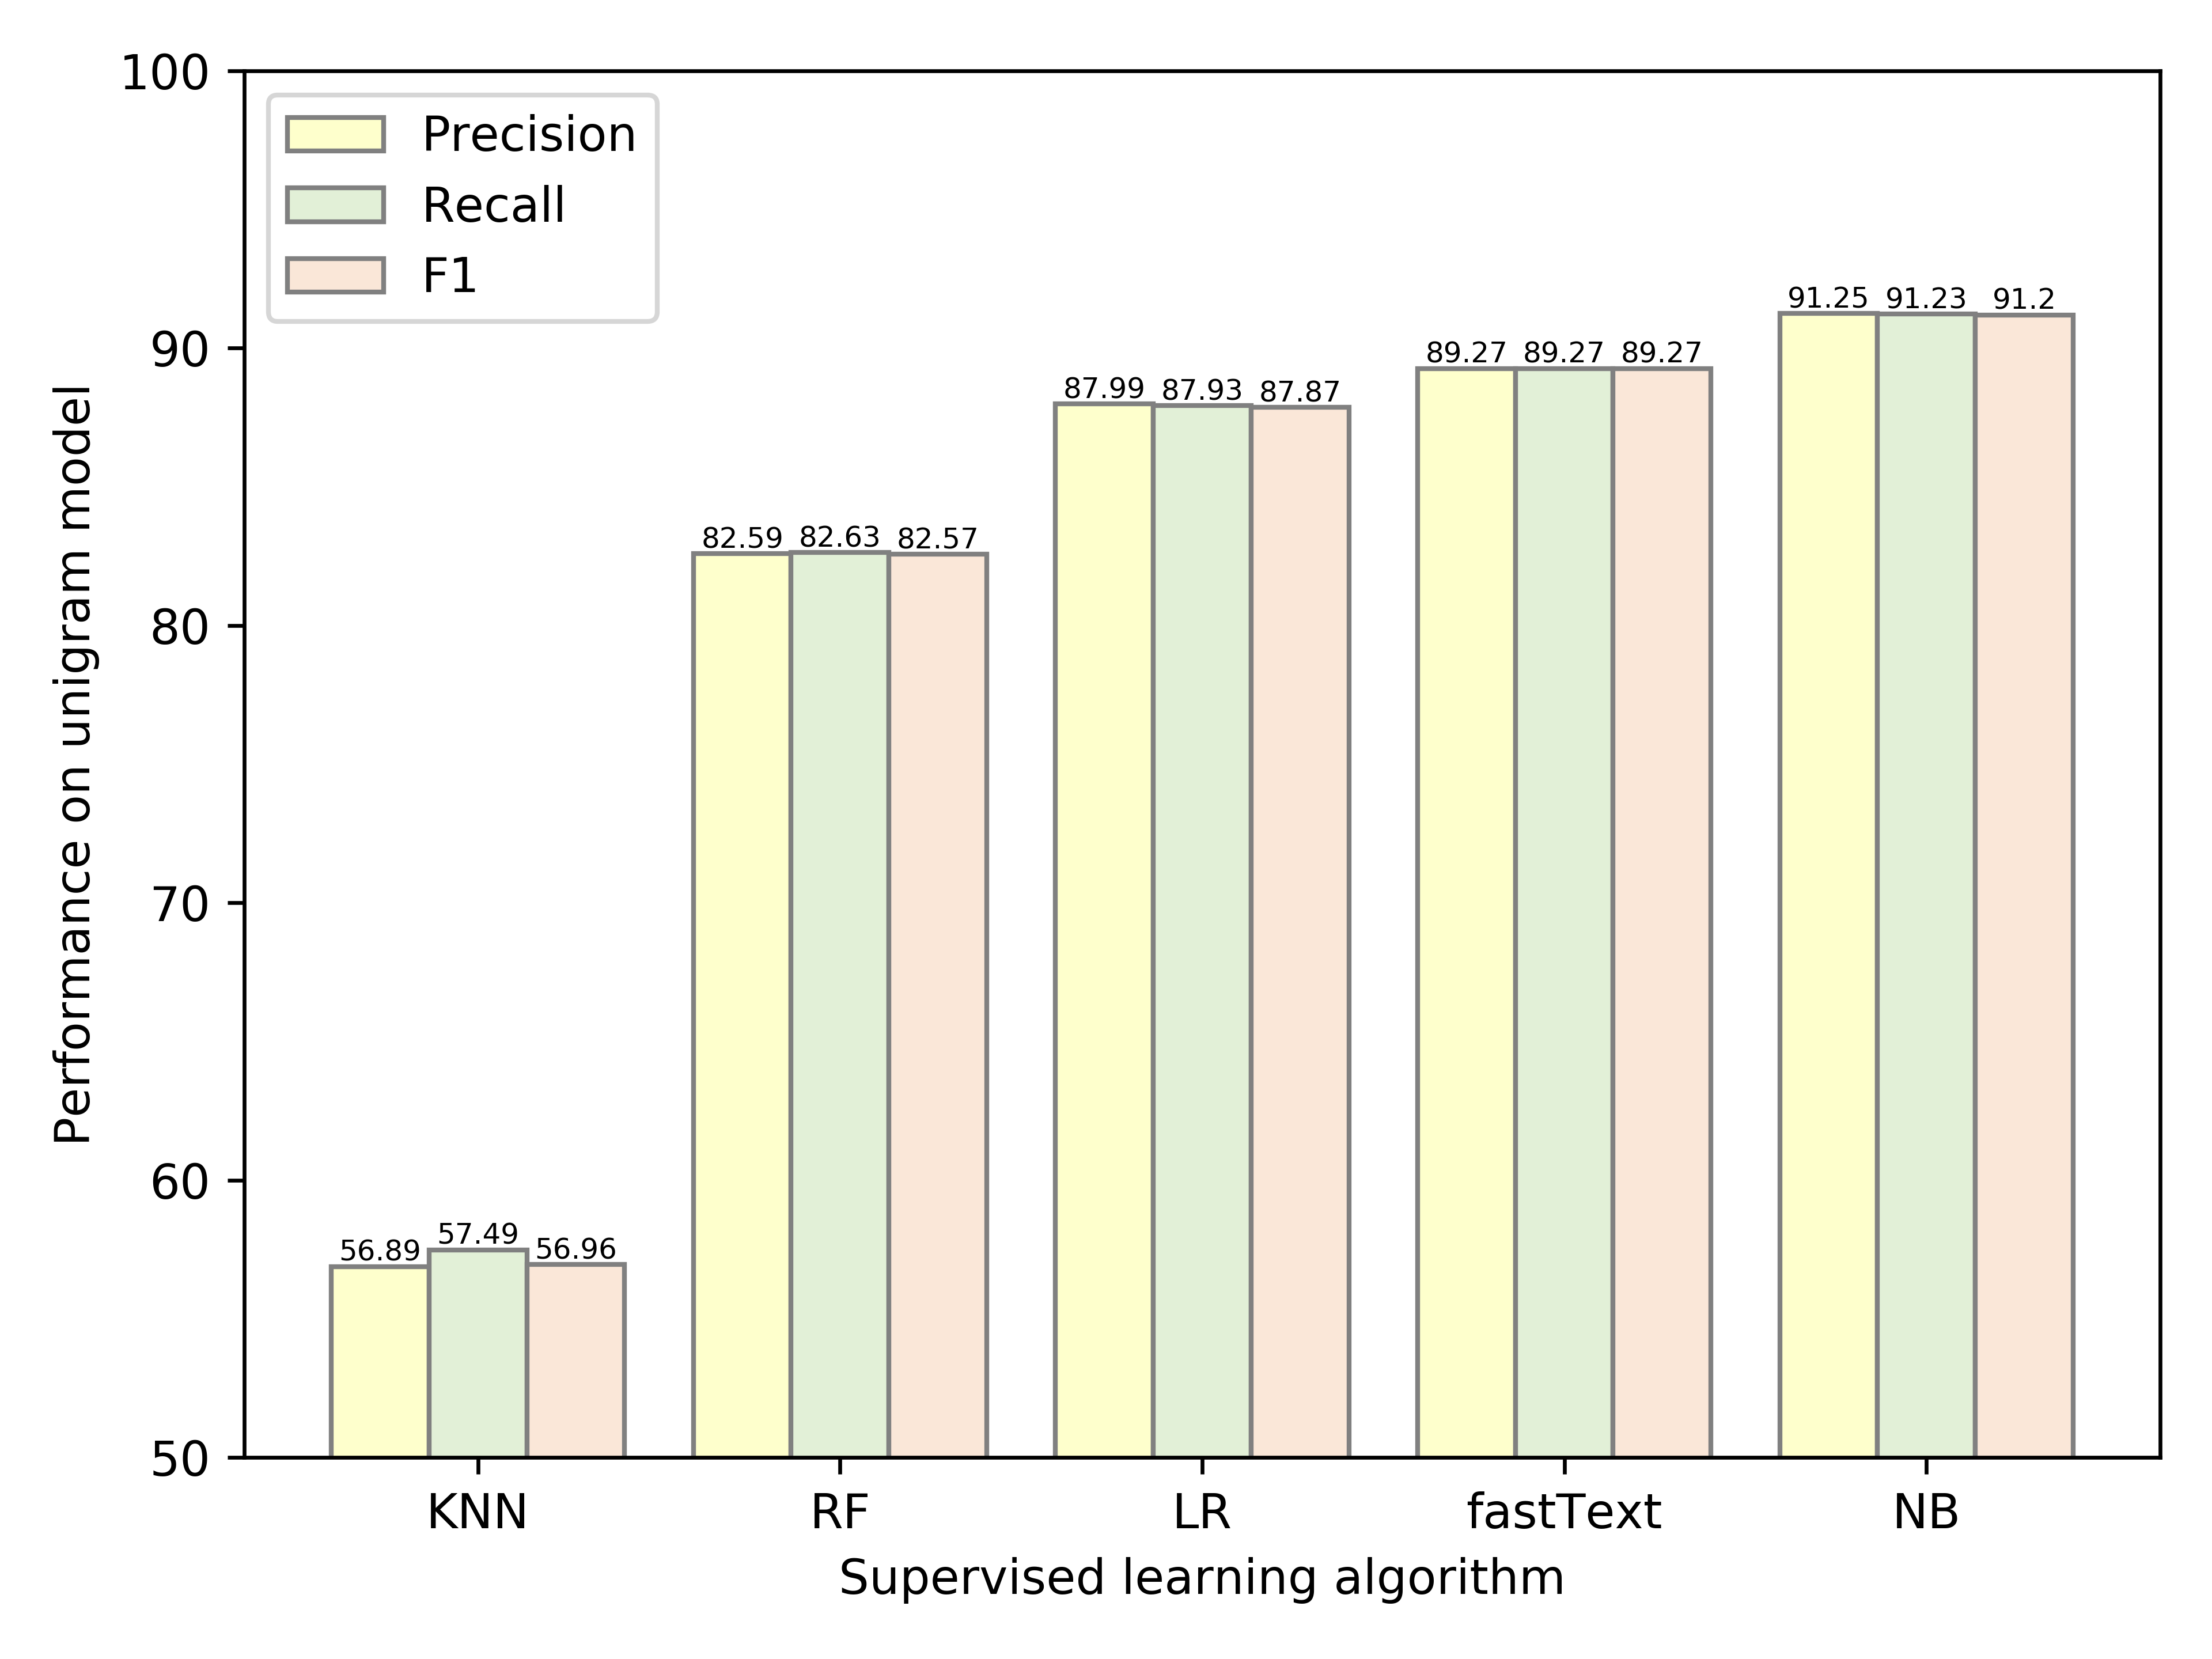
\includegraphics[width=0.40\textwidth]{images/unigram.png}}
\subfigure[bigrams]{
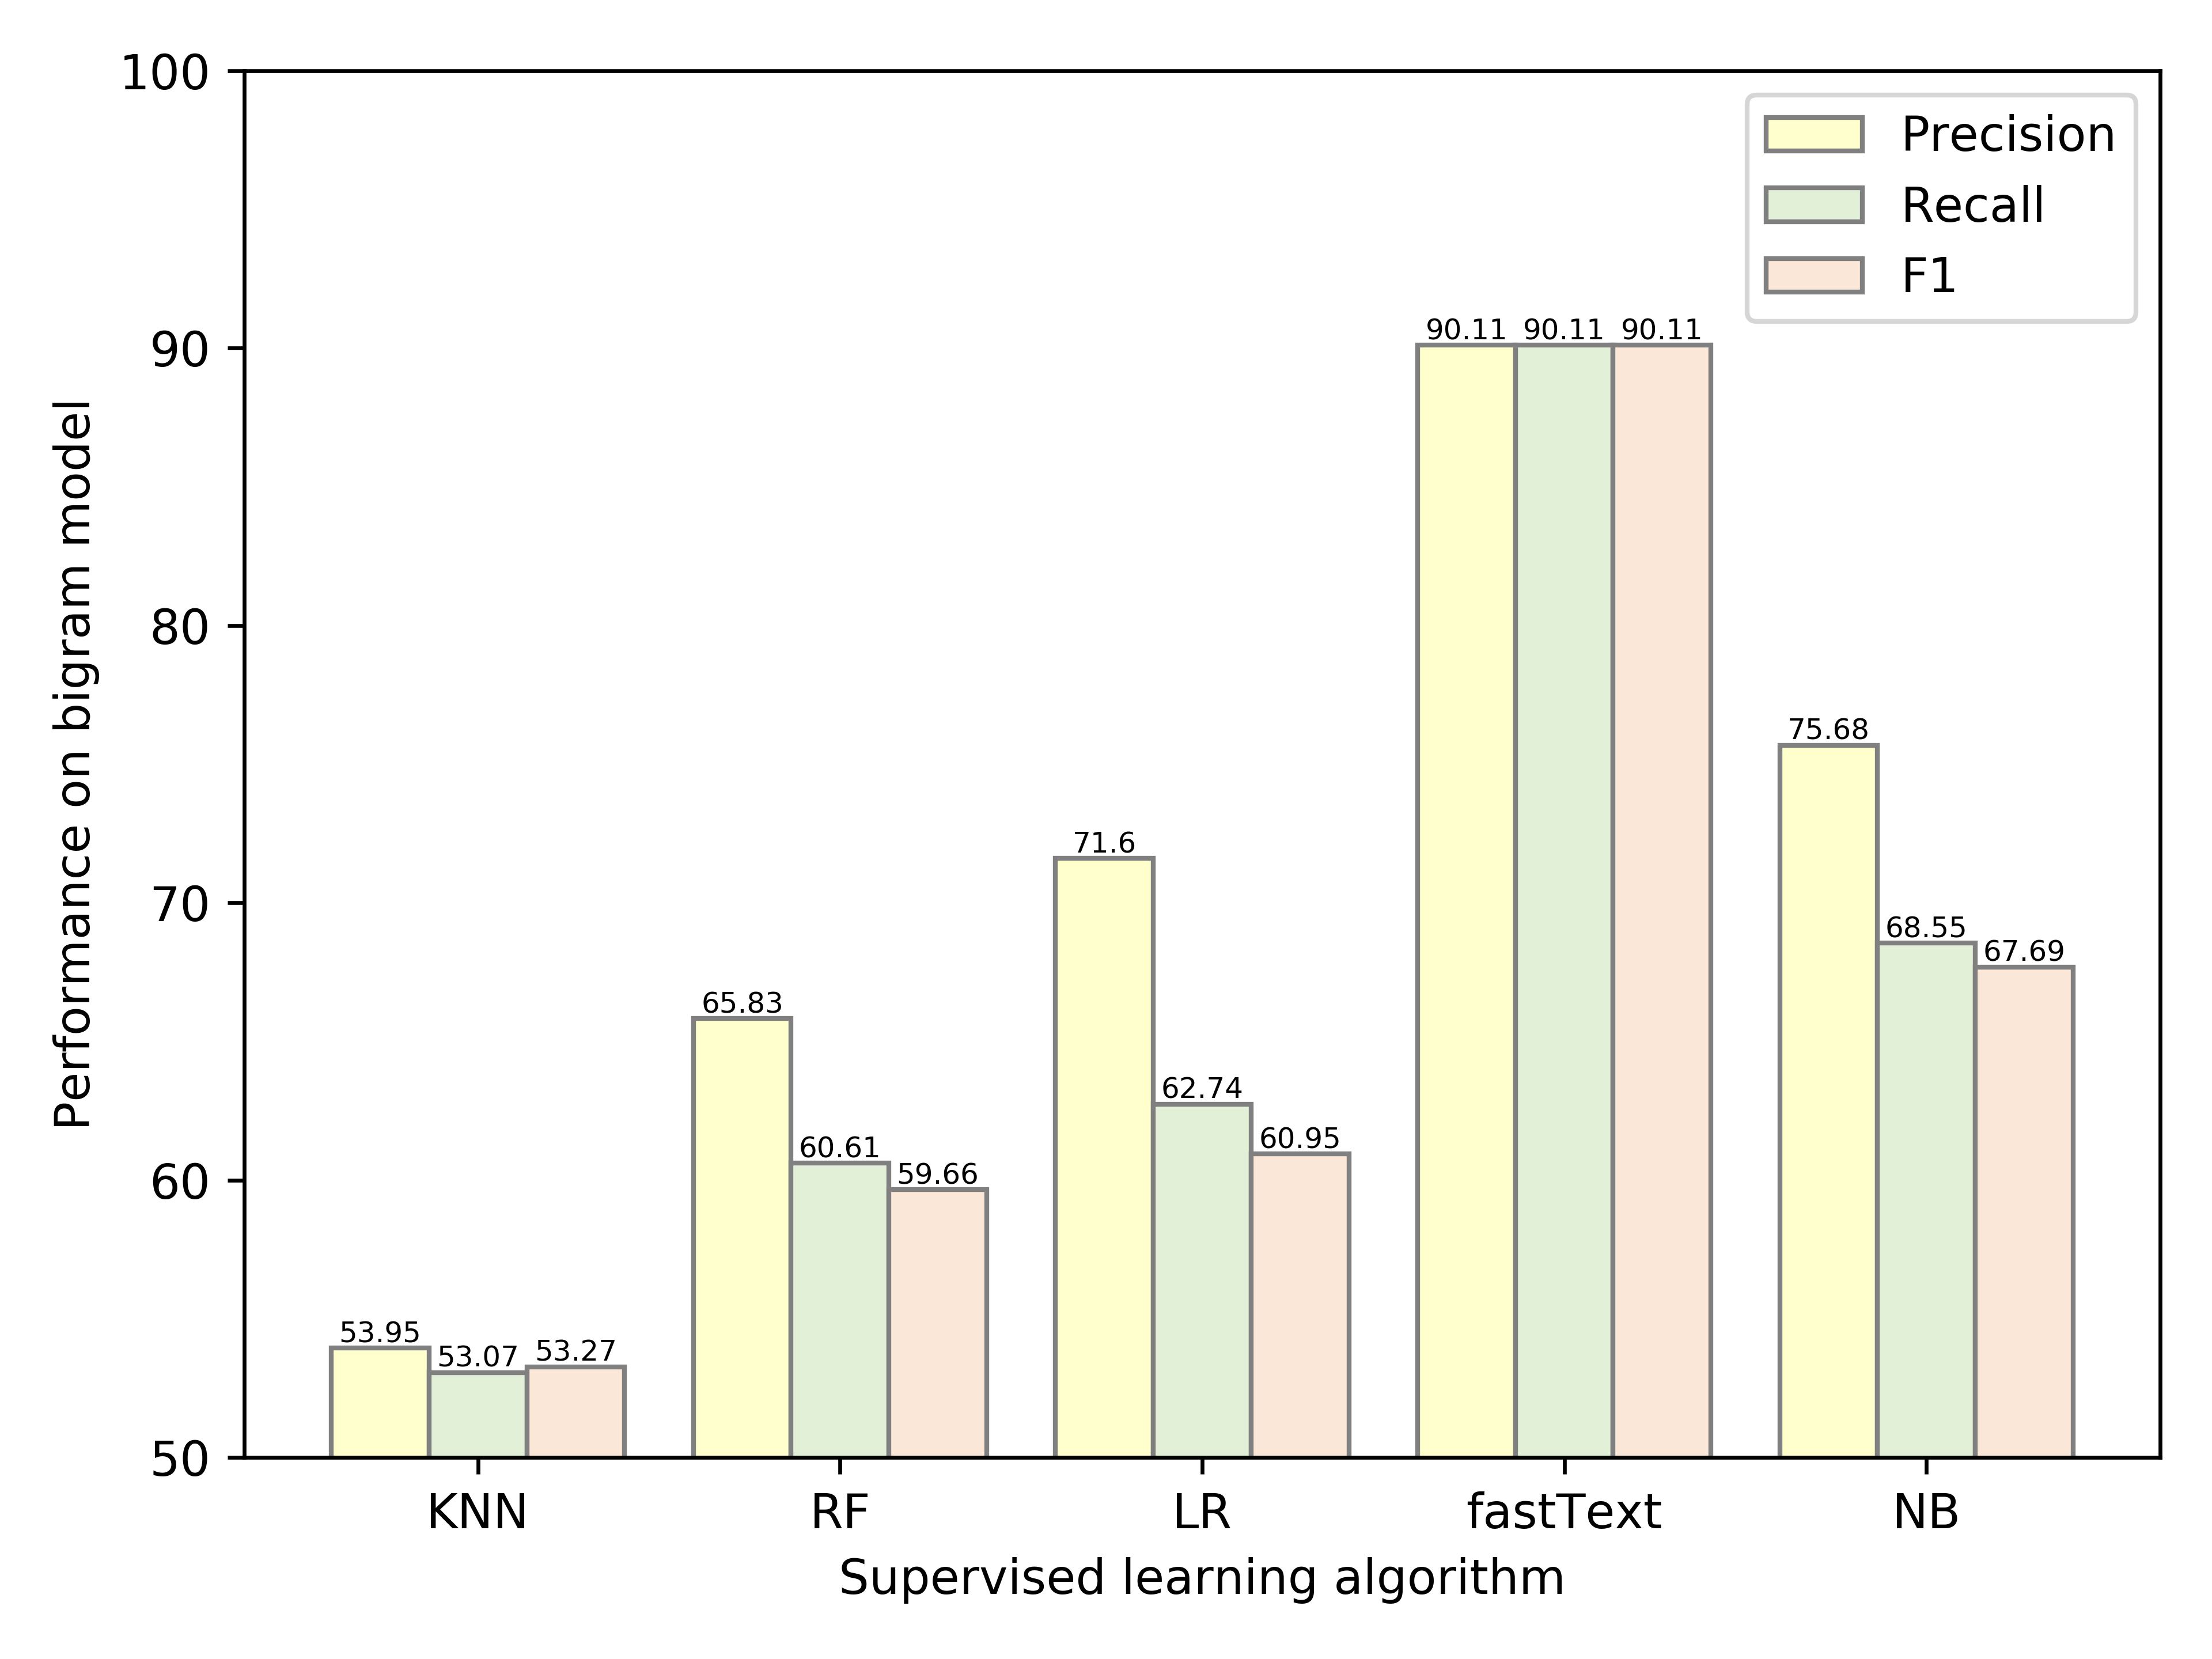
\includegraphics[width=0.40\textwidth]{images/bigram.png}}
\caption{Multi-model evaluation of corpus}
\label{fig:corpus-evaluation}
\end{figure}

\section{Platform Design and Demonstration}
Fig.~\ref{fig:Senti-weibo} depicts the architecture of Senti-weibo, which has two main function models: \textit{offline scripts} and \textit{front-end visualization}.

\textit{Offline scripts} model encapsulates scripts such as spider, corpus iteration, and text pre-processing. Fig.~\ref{fig:segmentation-tools-precision} shows the different performance of the model caused by different pre-processing rules. We take six Chinese segmentation tools to cut test dataset, and apply the pre-trained model segmented by jieba\footnote{\url{https://github.com/fxsjy/jieba}} to classify each test dataset. Jieba is not the best Chinese segmentation tool, but the consistent rules in the training and test environment maximize the performance of model.

\begin{figure}[htbp]
\vspace{-0.5cm}   %调整图片与上文的垂直距离
\centering
\begin{minipage}[t]{0.43\textwidth}
\centering
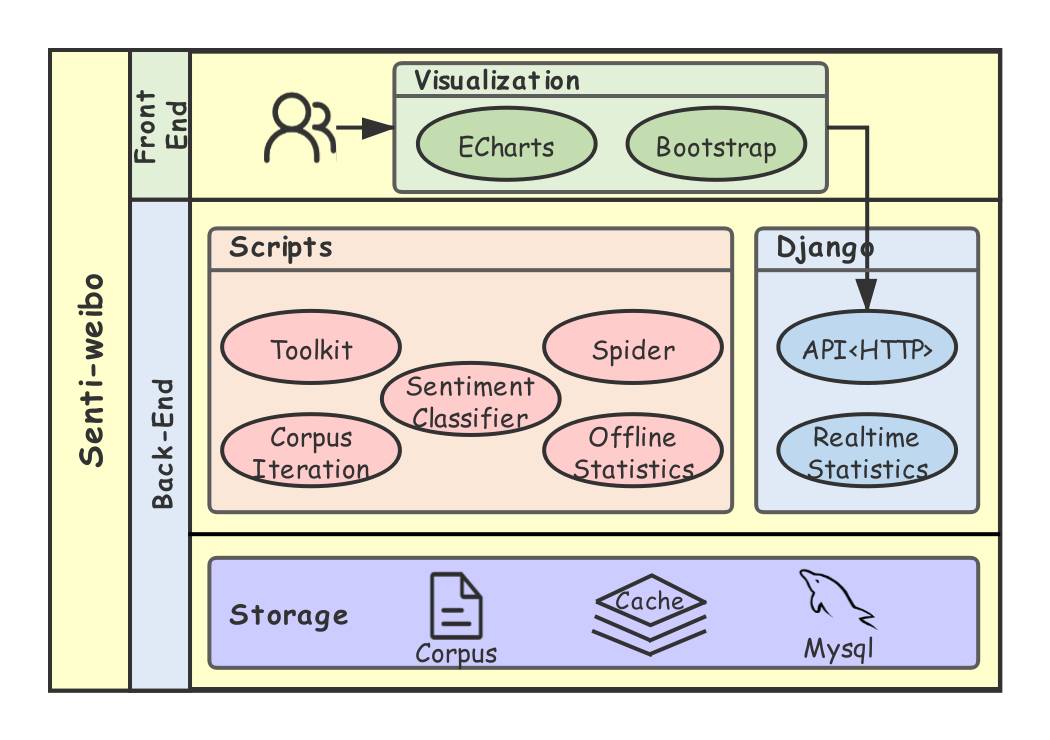
\includegraphics[width=5.2cm]{images/Architecture-of-Senti-weibo-3.png}
\caption{Architecture of Senti-weibo}
\label{fig:Senti-weibo}
\end{minipage}
\begin{minipage}[t]{0.43\textwidth}
\centering
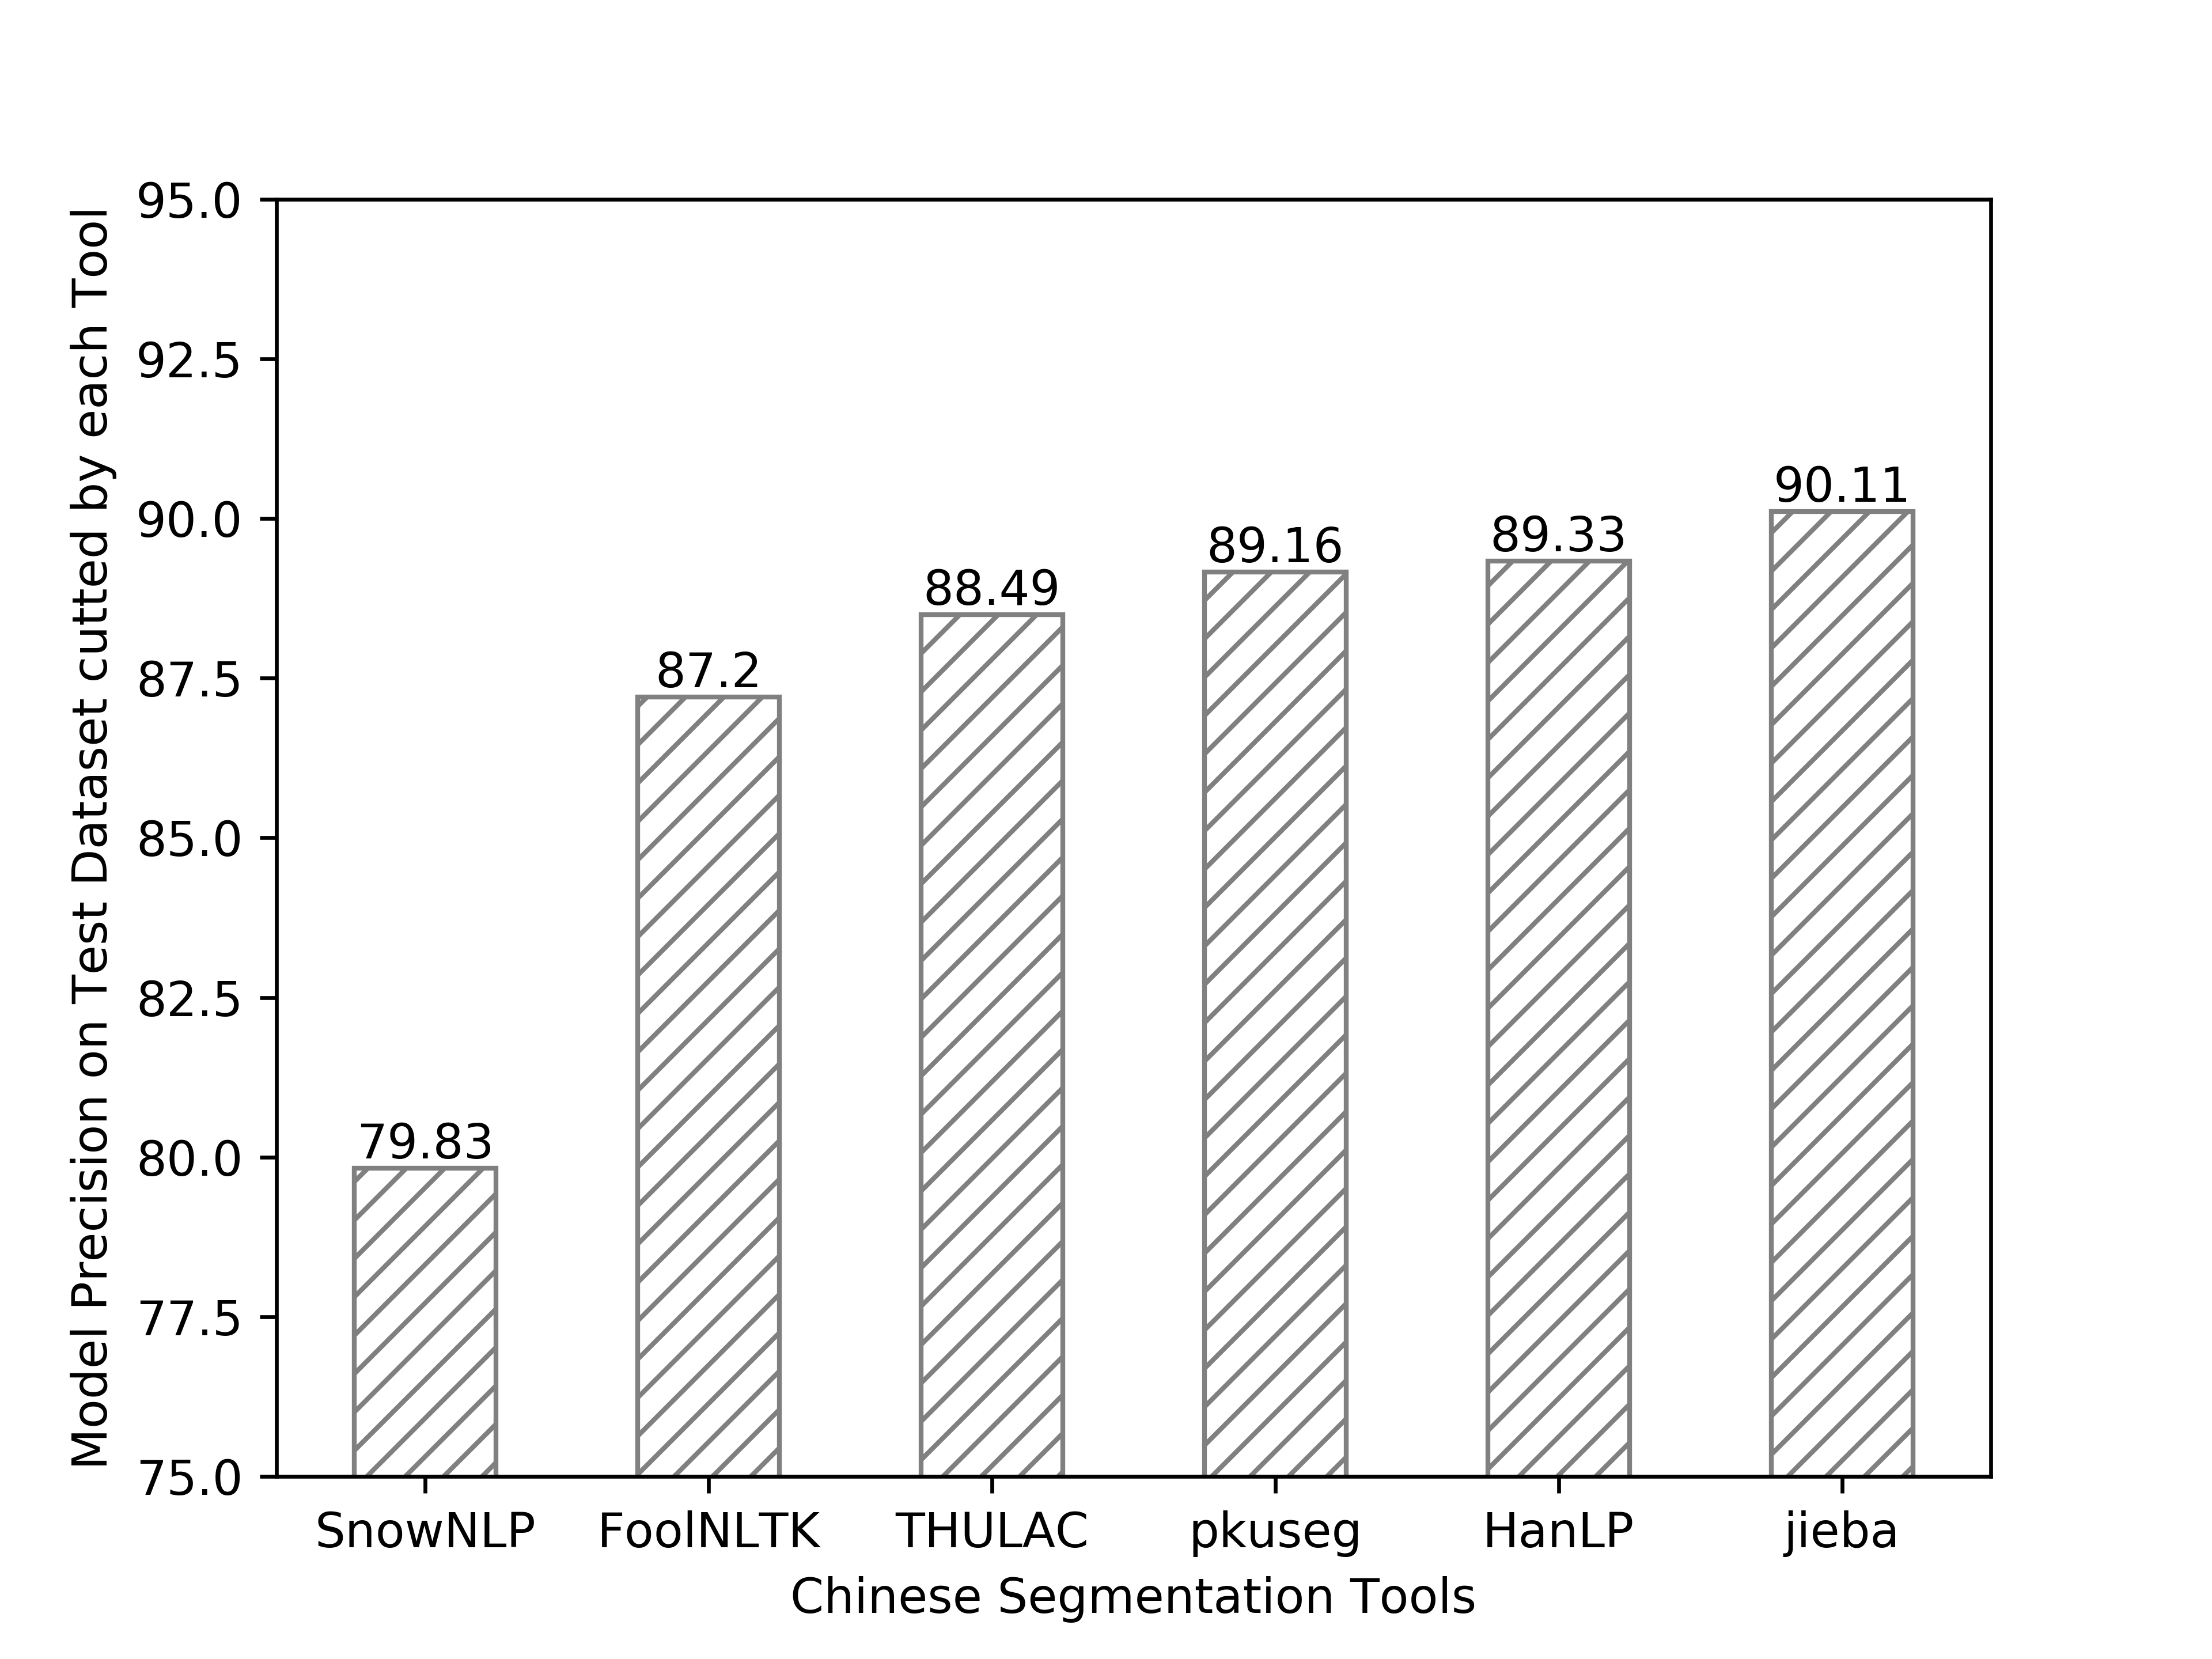
\includegraphics[width=5.2cm]{images/model-precision-on-test-dataset-cutted-by-each-tool.png}
\caption{Chinese segmentation tools}
\label{fig:segmentation-tools-precision}
\end{minipage}
\end{figure}

\textit{Front-end visualization} provides interface to interact with back-end. Fig.~\ref{fig:sentiment-trend} shows the results of platform's temporal sentiment analysis of two specified topics. Fig.~\ref{fig:huawei-1day} represents the daily sentiment trend of Huawei from March to July. The negative sentiment of Huawei since May 16 accurately reflects the event that Huawei is added to the Entity List. Fig.~\ref{fig:trade-5min} reflects the sentiment trend of China-US trade from May 29 to May 30 in a five-minutes frequency, which corresponds to the intense emotional changes of Chinese netizen to the anchors' debate between China and US. We also open-source weibos for two topics collected from April to July. More sentiment analysis of topic can be available by visiting Senti-weibo. 

\begin{figure}[ht]
\vspace{-0.5cm}  % 调整图片与上文的垂直距离
\centering  %图片全局居中
\subfigure[Huawei]{
\label{fig:huawei-1day}
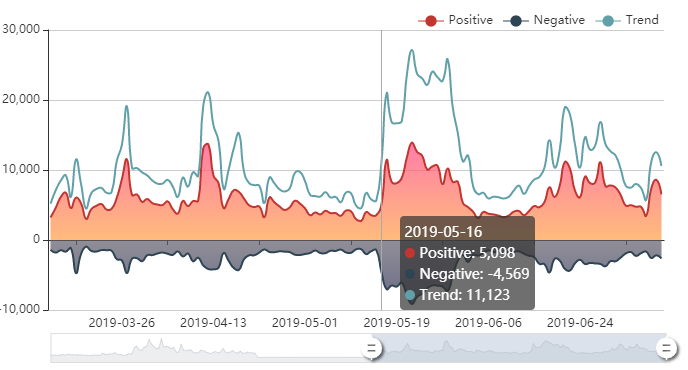
\includegraphics[width=0.40\textwidth]{images/huawei-alert.png}}
\subfigure[China-US trade]{
\label{fig:trade-5min}
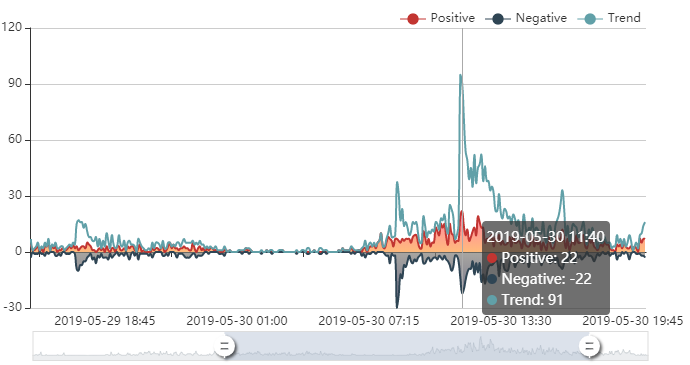
\includegraphics[width=0.40\textwidth]{images/china-us-detate-5min.png}}
\caption{Temporal sentiment analysis}
\label{fig:sentiment-trend}
\end{figure}

\section{Summary}
 % 文章篇幅、预处理工具的实现细节,平台的实现细节等各种细节。We also open-source weibo data for two topics collected from April to July。以构建语料库为中心,顺带 more details of corpus construction and  更多的细节,例如爬虫的设计、文本预处理工具的设计、情感分析平台的构建,
 In this work, we aim at the construction and iteration of Chinese Weibo sentiment analysis corpus. The details of Senti-weibo can be available on GitHub\footnote{https://github.com/wansho/senti-weibo}, including introduction video, design of pre-processing tool, implement of web demonstration and others.
 
\bibliographystyle{splncs04.bst}
\bibliography{mybibliography.bib}

\end{document}
